\PassOptionsToPackage{unicode=true}{hyperref} % options for packages loaded elsewhere
\PassOptionsToPackage{hyphens}{url}
%
\documentclass[]{article}
\usepackage{lmodern}
\usepackage{amssymb,amsmath}
\usepackage{ifxetex,ifluatex}
\usepackage{fixltx2e} % provides \textsubscript
\usepackage[T1]{fontenc}
\usepackage[utf8]{inputenc}
\usepackage{textcomp} % provides euro and other symbols
% use upquote if available, for straight quotes in verbatim environments
\IfFileExists{upquote.sty}{\usepackage{upquote}}{}
% use microtype if available
\IfFileExists{microtype.sty}{%
\usepackage[]{microtype}
\UseMicrotypeSet[protrusion]{basicmath} % disable protrusion for tt fonts
}{}
\IfFileExists{parskip.sty}{%
\usepackage{parskip}
}{% else
\setlength{\parindent}{0pt}
\setlength{\parskip}{6pt plus 2pt minus 1pt}
}
\usepackage{hyperref}
\hypersetup{
    colorlinks=true,
    linkcolor=blue,
    filecolor=magenta,
    urlcolor=cyan,
}
\urlstyle{same}  % don't use monospace font for urls
\usepackage{color}
\usepackage{fancyvrb}
\newcommand{\VerbBar}{|}
\newcommand{\VERB}{\Verb[commandchars=\\\{\}]}
\DefineVerbatimEnvironment{Highlighting}{Verbatim}{commandchars=\\\{\}}
% Add ',fontsize=\small' for more characters per line
\newenvironment{Shaded}{}{}
\newcommand{\KeywordTok}[1]{\textcolor[rgb]{0.00,0.44,0.13}{\textbf{#1}}}
\newcommand{\DataTypeTok}[1]{\textcolor[rgb]{0.56,0.13,0.00}{#1}}
\newcommand{\DecValTok}[1]{\textcolor[rgb]{0.25,0.63,0.44}{#1}}
\newcommand{\BaseNTok}[1]{\textcolor[rgb]{0.25,0.63,0.44}{#1}}
\newcommand{\FloatTok}[1]{\textcolor[rgb]{0.25,0.63,0.44}{#1}}
\newcommand{\ConstantTok}[1]{\textcolor[rgb]{0.53,0.00,0.00}{#1}}
\newcommand{\CharTok}[1]{\textcolor[rgb]{0.25,0.44,0.63}{#1}}
\newcommand{\SpecialCharTok}[1]{\textcolor[rgb]{0.25,0.44,0.63}{#1}}
\newcommand{\StringTok}[1]{\textcolor[rgb]{0.25,0.44,0.63}{#1}}
\newcommand{\VerbatimStringTok}[1]{\textcolor[rgb]{0.25,0.44,0.63}{#1}}
\newcommand{\SpecialStringTok}[1]{\textcolor[rgb]{0.73,0.40,0.53}{#1}}
\newcommand{\ImportTok}[1]{#1}
\newcommand{\CommentTok}[1]{\textcolor[rgb]{0.38,0.63,0.69}{\textit{#1}}}
\newcommand{\DocumentationTok}[1]{\textcolor[rgb]{0.73,0.13,0.13}{\textit{#1}}}
\newcommand{\AnnotationTok}[1]{\textcolor[rgb]{0.38,0.63,0.69}{\textbf{\textit{#1}}}}
\newcommand{\CommentVarTok}[1]{\textcolor[rgb]{0.38,0.63,0.69}{\textbf{\textit{#1}}}}
\newcommand{\OtherTok}[1]{\textcolor[rgb]{0.00,0.44,0.13}{#1}}
\newcommand{\FunctionTok}[1]{\textcolor[rgb]{0.02,0.16,0.49}{#1}}
\newcommand{\VariableTok}[1]{\textcolor[rgb]{0.10,0.09,0.49}{#1}}
\newcommand{\ControlFlowTok}[1]{\textcolor[rgb]{0.00,0.44,0.13}{\textbf{#1}}}
\newcommand{\OperatorTok}[1]{\textcolor[rgb]{0.40,0.40,0.40}{#1}}
\newcommand{\BuiltInTok}[1]{#1}
\newcommand{\ExtensionTok}[1]{#1}
\newcommand{\PreprocessorTok}[1]{\textcolor[rgb]{0.74,0.48,0.00}{#1}}
\newcommand{\AttributeTok}[1]{\textcolor[rgb]{0.49,0.56,0.16}{#1}}
\newcommand{\RegionMarkerTok}[1]{#1}
\newcommand{\InformationTok}[1]{\textcolor[rgb]{0.38,0.63,0.69}{\textbf{\textit{#1}}}}
\newcommand{\WarningTok}[1]{\textcolor[rgb]{0.38,0.63,0.69}{\textbf{\textit{#1}}}}
\newcommand{\AlertTok}[1]{\textcolor[rgb]{1.00,0.00,0.00}{\textbf{#1}}}
\newcommand{\ErrorTok}[1]{\textcolor[rgb]{1.00,0.00,0.00}{\textbf{#1}}}
\newcommand{\NormalTok}[1]{#1}
\usepackage{longtable,booktabs}
% Fix footnotes in tables (requires footnote package)
\IfFileExists{footnote.sty}{\usepackage{footnote}\makesavenoteenv{longtable}}{}
\usepackage{graphicx,grffile}
\graphicspath{{../assets/}{../renderings/}{../schematics/}}
\usepackage{subfig}
\usepackage{float}
\makeatletter
\def\maxwidth{\ifdim\Gin@nat@width>\linewidth\linewidth\else\Gin@nat@width\fi}
\def\maxheight{\ifdim\Gin@nat@height>\textheight\textheight\else\Gin@nat@height\fi}
\makeatother
% Scale images if necessary, so that they will not overflow the page
% margins by default, and it is still possible to overwrite the defaults
% using explicit options in \includegraphics[width, height, ...]{}
\setkeys{Gin}{width=\maxwidth,height=\maxheight,keepaspectratio}
\setlength{\emergencystretch}{3em}  % prevent overfull lines
\providecommand{\tightlist}{%
  \setlength{\itemsep}{0pt}\setlength{\parskip}{0pt}}
\setcounter{secnumdepth}{0}
% Redefines (sub)paragraphs to behave more like sections
\ifx\paragraph\undefined\else
\let\oldparagraph\paragraph
\renewcommand{\paragraph}[1]{\oldparagraph{#1}\mbox{}}
\fi
\ifx\subparagraph\undefined\else
\let\oldsubparagraph\subparagraph
\renewcommand{\subparagraph}[1]{\oldsubparagraph{#1}\mbox{}}
\fi

\title{Blue Hunters: Bluetooth RSSI Locator Robots}
\author{Jacob Glueck (\href{mailto:jng55@cornell.edu}{jng55}) \and Jane Du (\href{mailto:zd53@cornell.edu}{zd53}) \and Justin Cray (\href{mailto:jgc232@cornell.edu}{jgc232})}
\date{December 6, 2017}

\begin{document}
\maketitle

\hypertarget{introduction}{%
\subsection{Introduction}\label{introduction}}

Position estimation and navigation for indoor robots is an interesting problem.
In this article, we investigate using the Received Signal Strength Indicator (RSSI) of Bluetooth Low Energy (BLE) 4.0 chips to allow wheeled mobile robots to navigate towards a stationary base station.
Each robot was controlled by a PIC32MX250 microcontroller, and used a 3 axis magnetometer as as compass in order to reliably turn, as well as 2 micro 9 g servos to drive.
Each unit was powered with 3 AA batteries.
Finally, the chassis and wheels of each car were 3D printed.
Figure \ref{fig:robotsystem} shows the entire system.

\begin{figure}
  \centering
  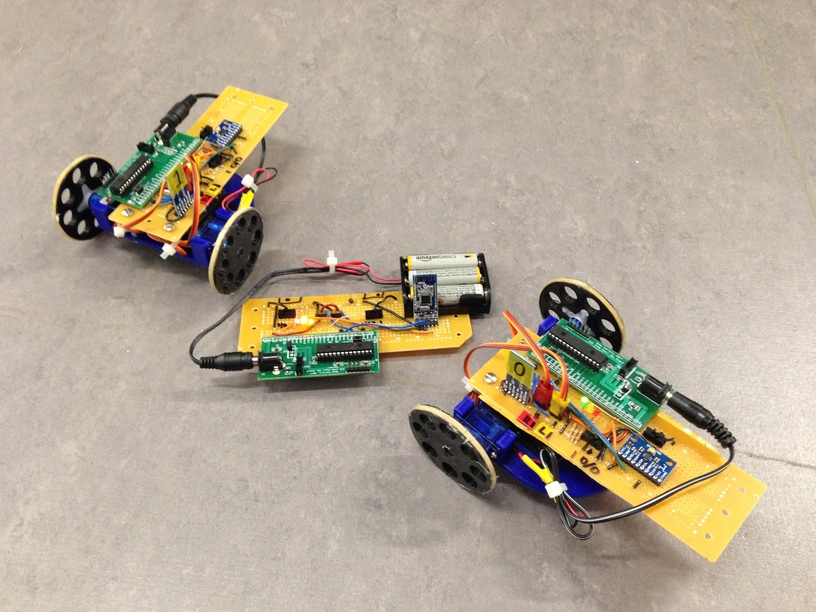
\includegraphics[width=0.8\textwidth]{full_system.jpg}
  \caption{Full system with 2 robots and the base station}
  \label{fig:robotsystem}
\end{figure}

\hypertarget{design}{%
\subsection{Design}\label{design}}

\hypertarget{chassis}{%
\subsubsection{Chassis}\label{chassis}}

The robots are made from 4 3D printed pieces: 2 wheels, the frame, and
the caster in the back.
Figure \ref{fig:robotchassis} shows the main components.
The servos, a 3 AA battery holder, and a perfboard containing all the circuitry are mounted directly to the frame.

\begin{figure}
  \centering
  \subfloat[Frame] {
    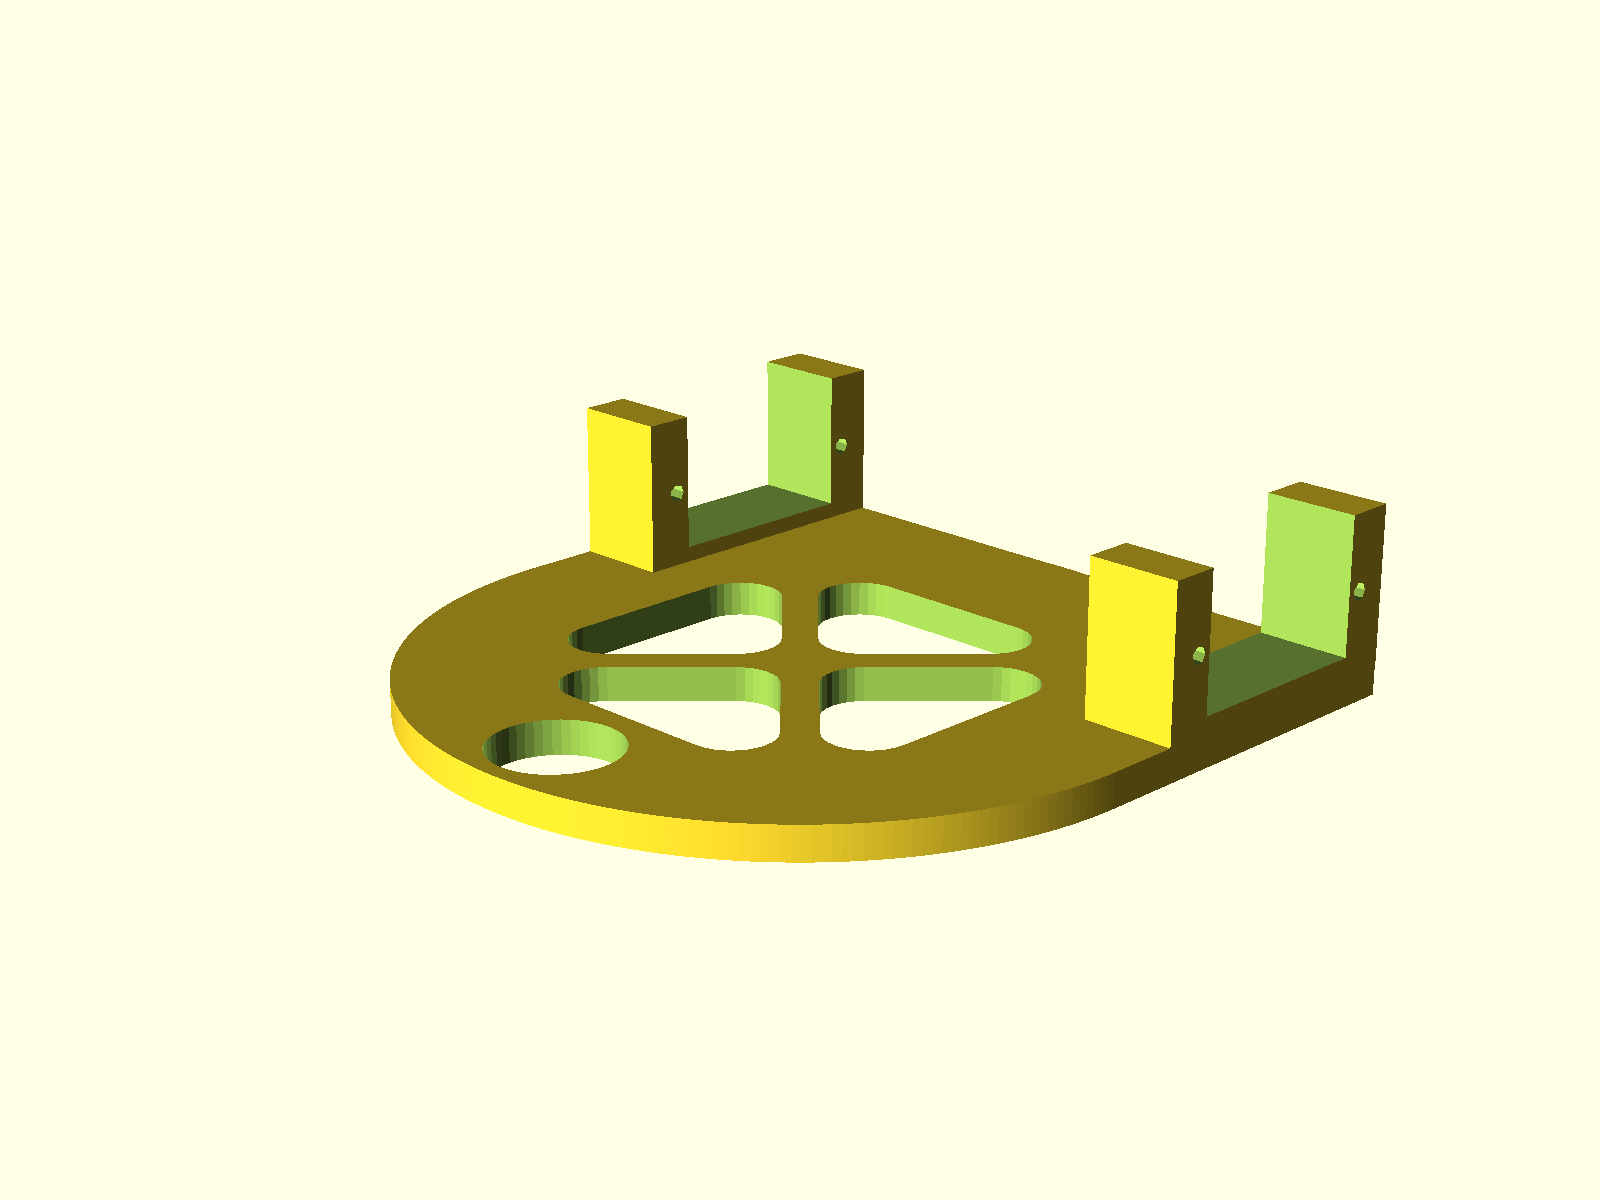
\includegraphics[width=0.5\textwidth,height=\textheight]{frame.png}
    \label{fig:robotfrane}
  }
  \subfloat[Wheel]{
    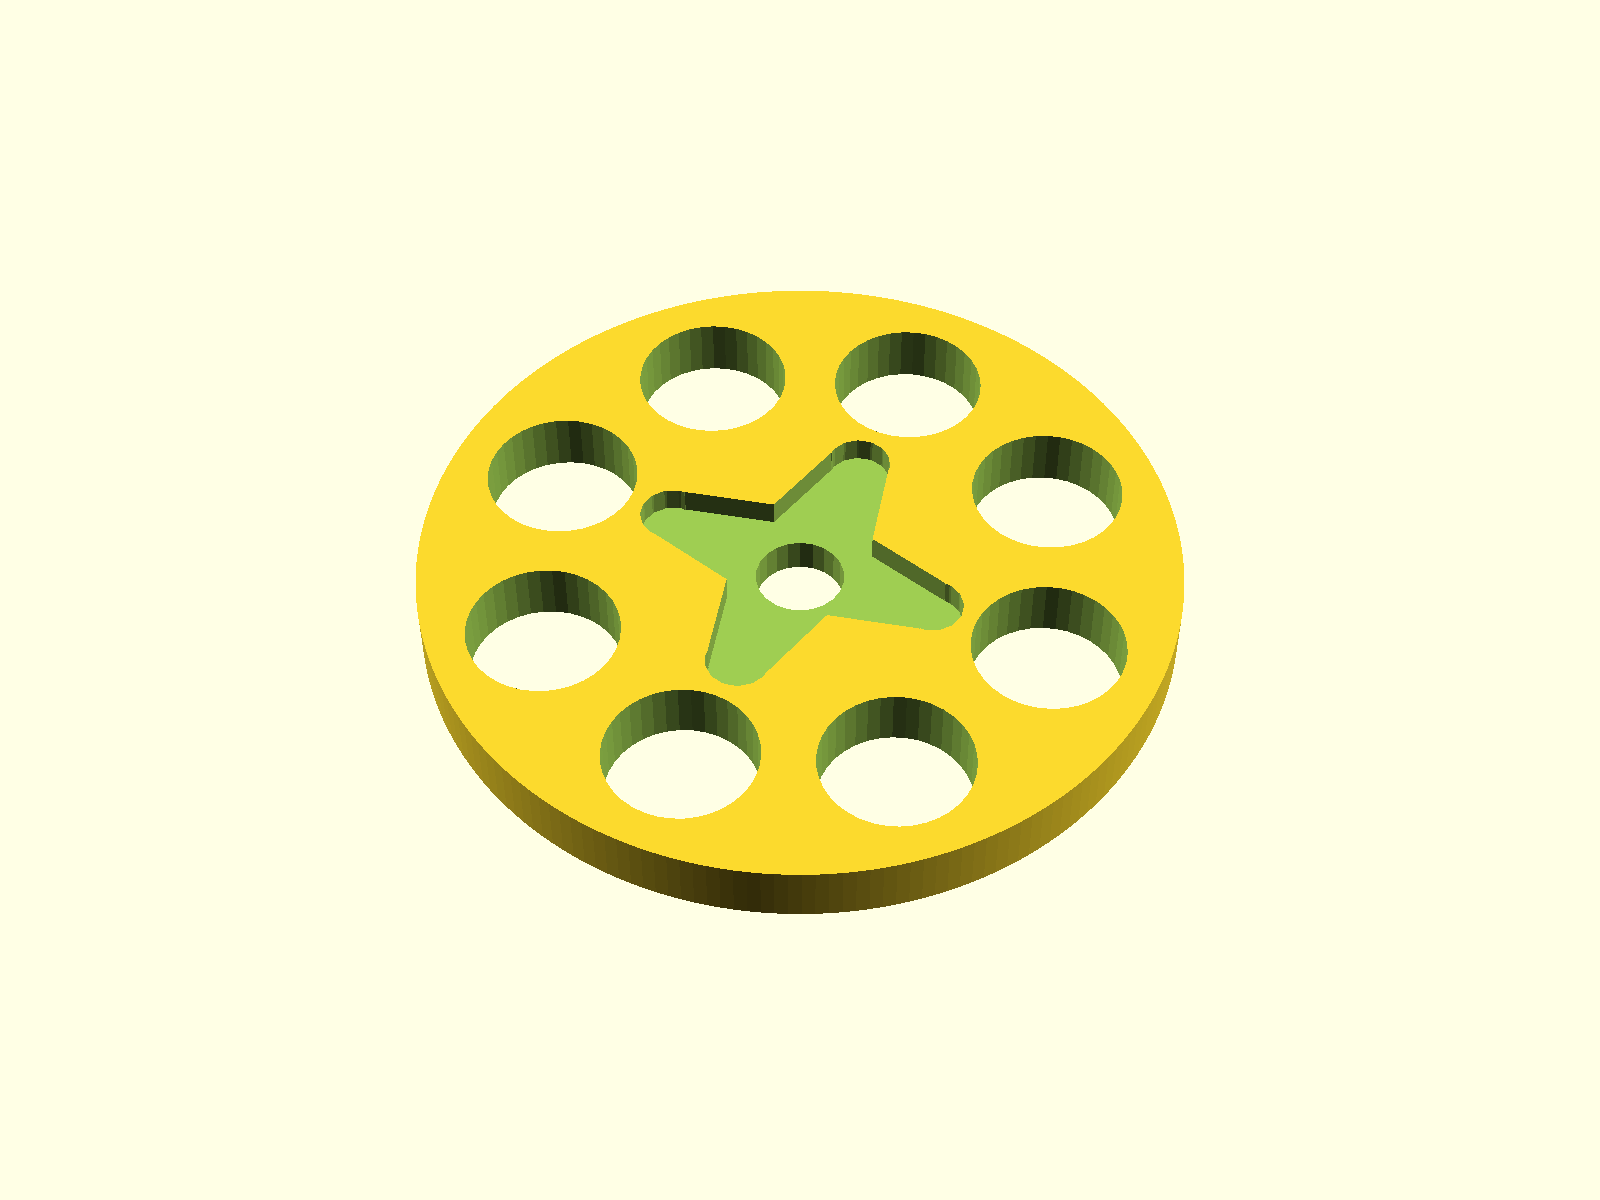
\includegraphics[width=0.5\textwidth,height=\textheight]{wheel.png}
    \label{fig:robotwheel}
  }
  \\
  \subfloat[Caster]{
    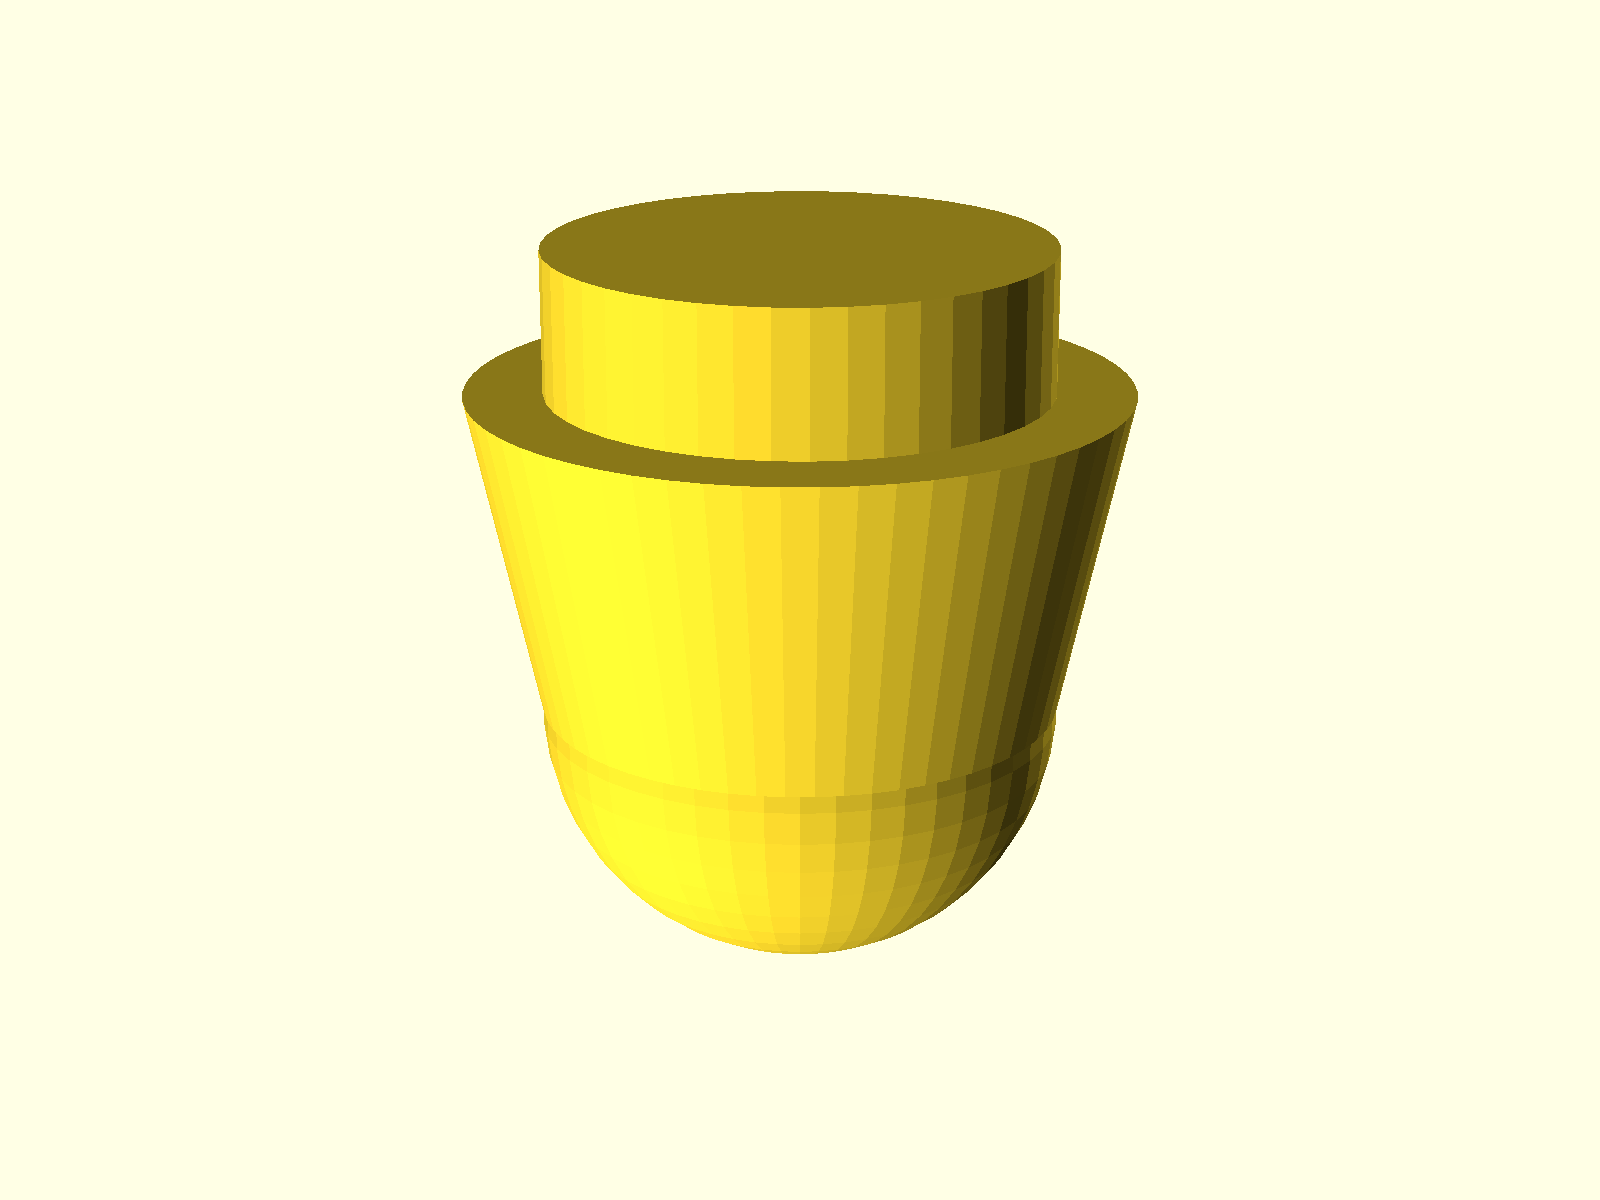
\includegraphics[width=0.5\textwidth,height=\textheight]{drag.png}
    \label{fig:robotcaster}
  }
  \caption{Components of robot chassis}
  \label{fig:robotchassis}
\end{figure}

The parts were printed in ABS using Maker Select 3D Printer v2 printers.
All parts were printed with a layer height of 0.3 mm, as there was no need for a smooth finish or high tolerances.
The parts where sliced with Cura.

\begin{figure}
  \centering
  \subfloat[Top view]{
    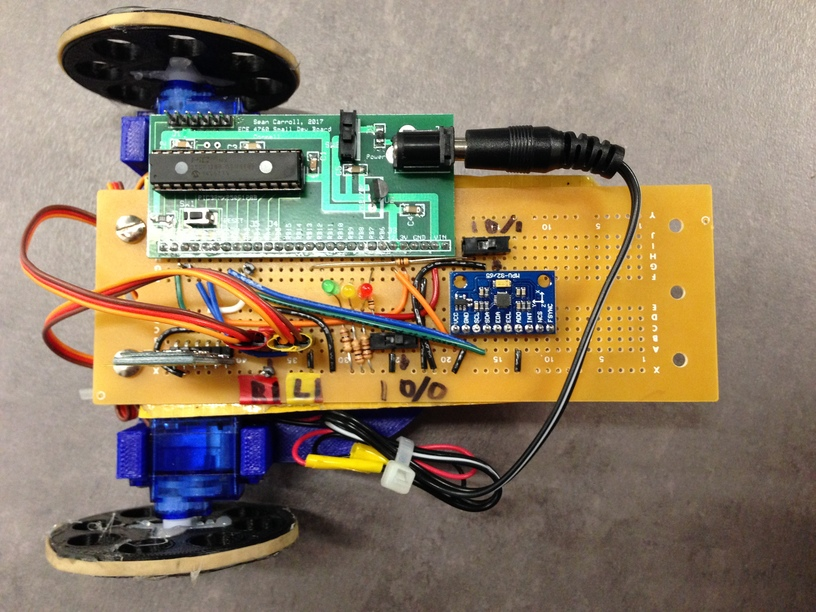
\includegraphics[width=0.5\textwidth]{top_view.jpg}
    \label{fig:robottop}
  }
  \subfloat[Side view]{
    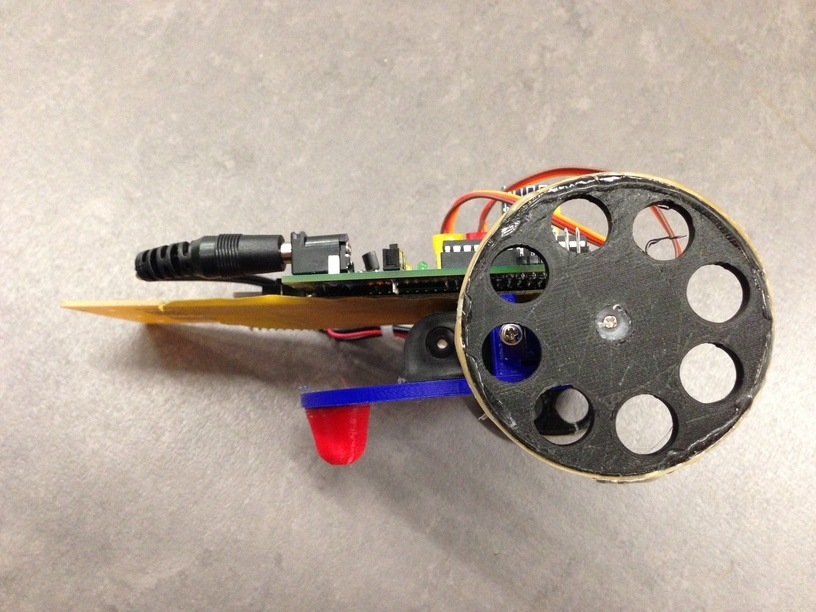
\includegraphics[width=0.5\textwidth]{side_view.jpg}
    \label{fig:robotside}
  }
  \\
  \subfloat[Front view]{
    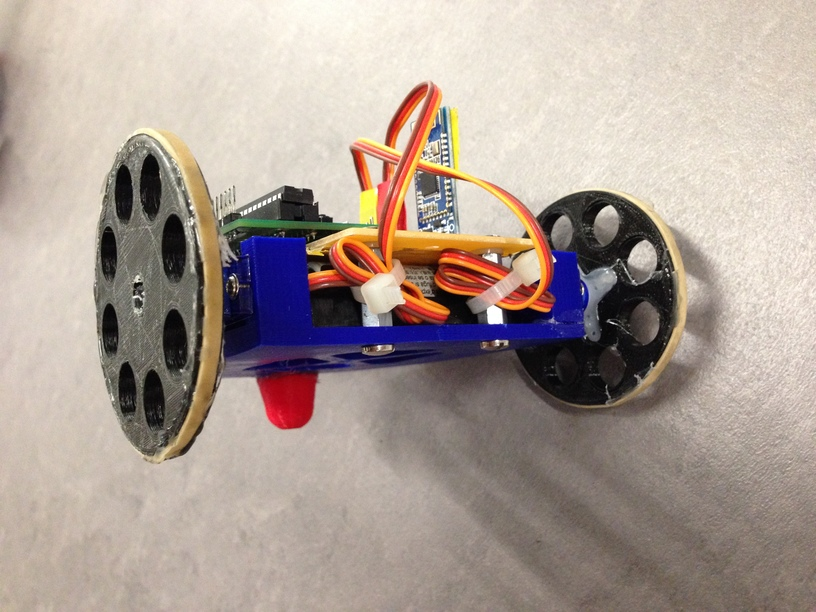
\includegraphics[width=0.5\textwidth]{front_view.jpg}
    \label{fig:robotfront}
  }
  \subfloat[Back view]{
    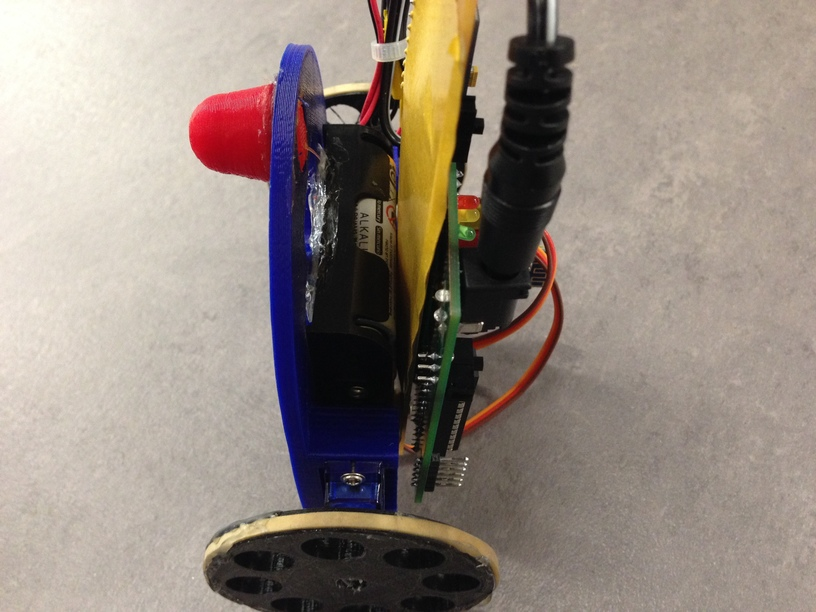
\includegraphics[width=0.5\textwidth]{inside_view.jpg}
    \label{fig:robotback}
  }
  \caption{Multiple views of the completed robots}
  \label{fig:robotviews}
\end{figure}

\hypertarget{electronics}{%
\subsubsection{Electronics}\label{electronics}}

Each robot consisted of 4 main components:
\begin{enumerate}
  \item PIC32MC250F128B microcontroller.
  \item MPU-9250 IMU with a 3 axis gryoscope, accelerometer, and magnetometer.
  \item HM-10 BLE module with a Texas Instruments CC2541 chip.
  \item Two 9 gram FS90R micro continuous rotation servos.
\end{enumerate}

The components are connected as shown in figure \ref{fig:schematic}.

\begin{figure}
  \centering
  \subfloat[] {
    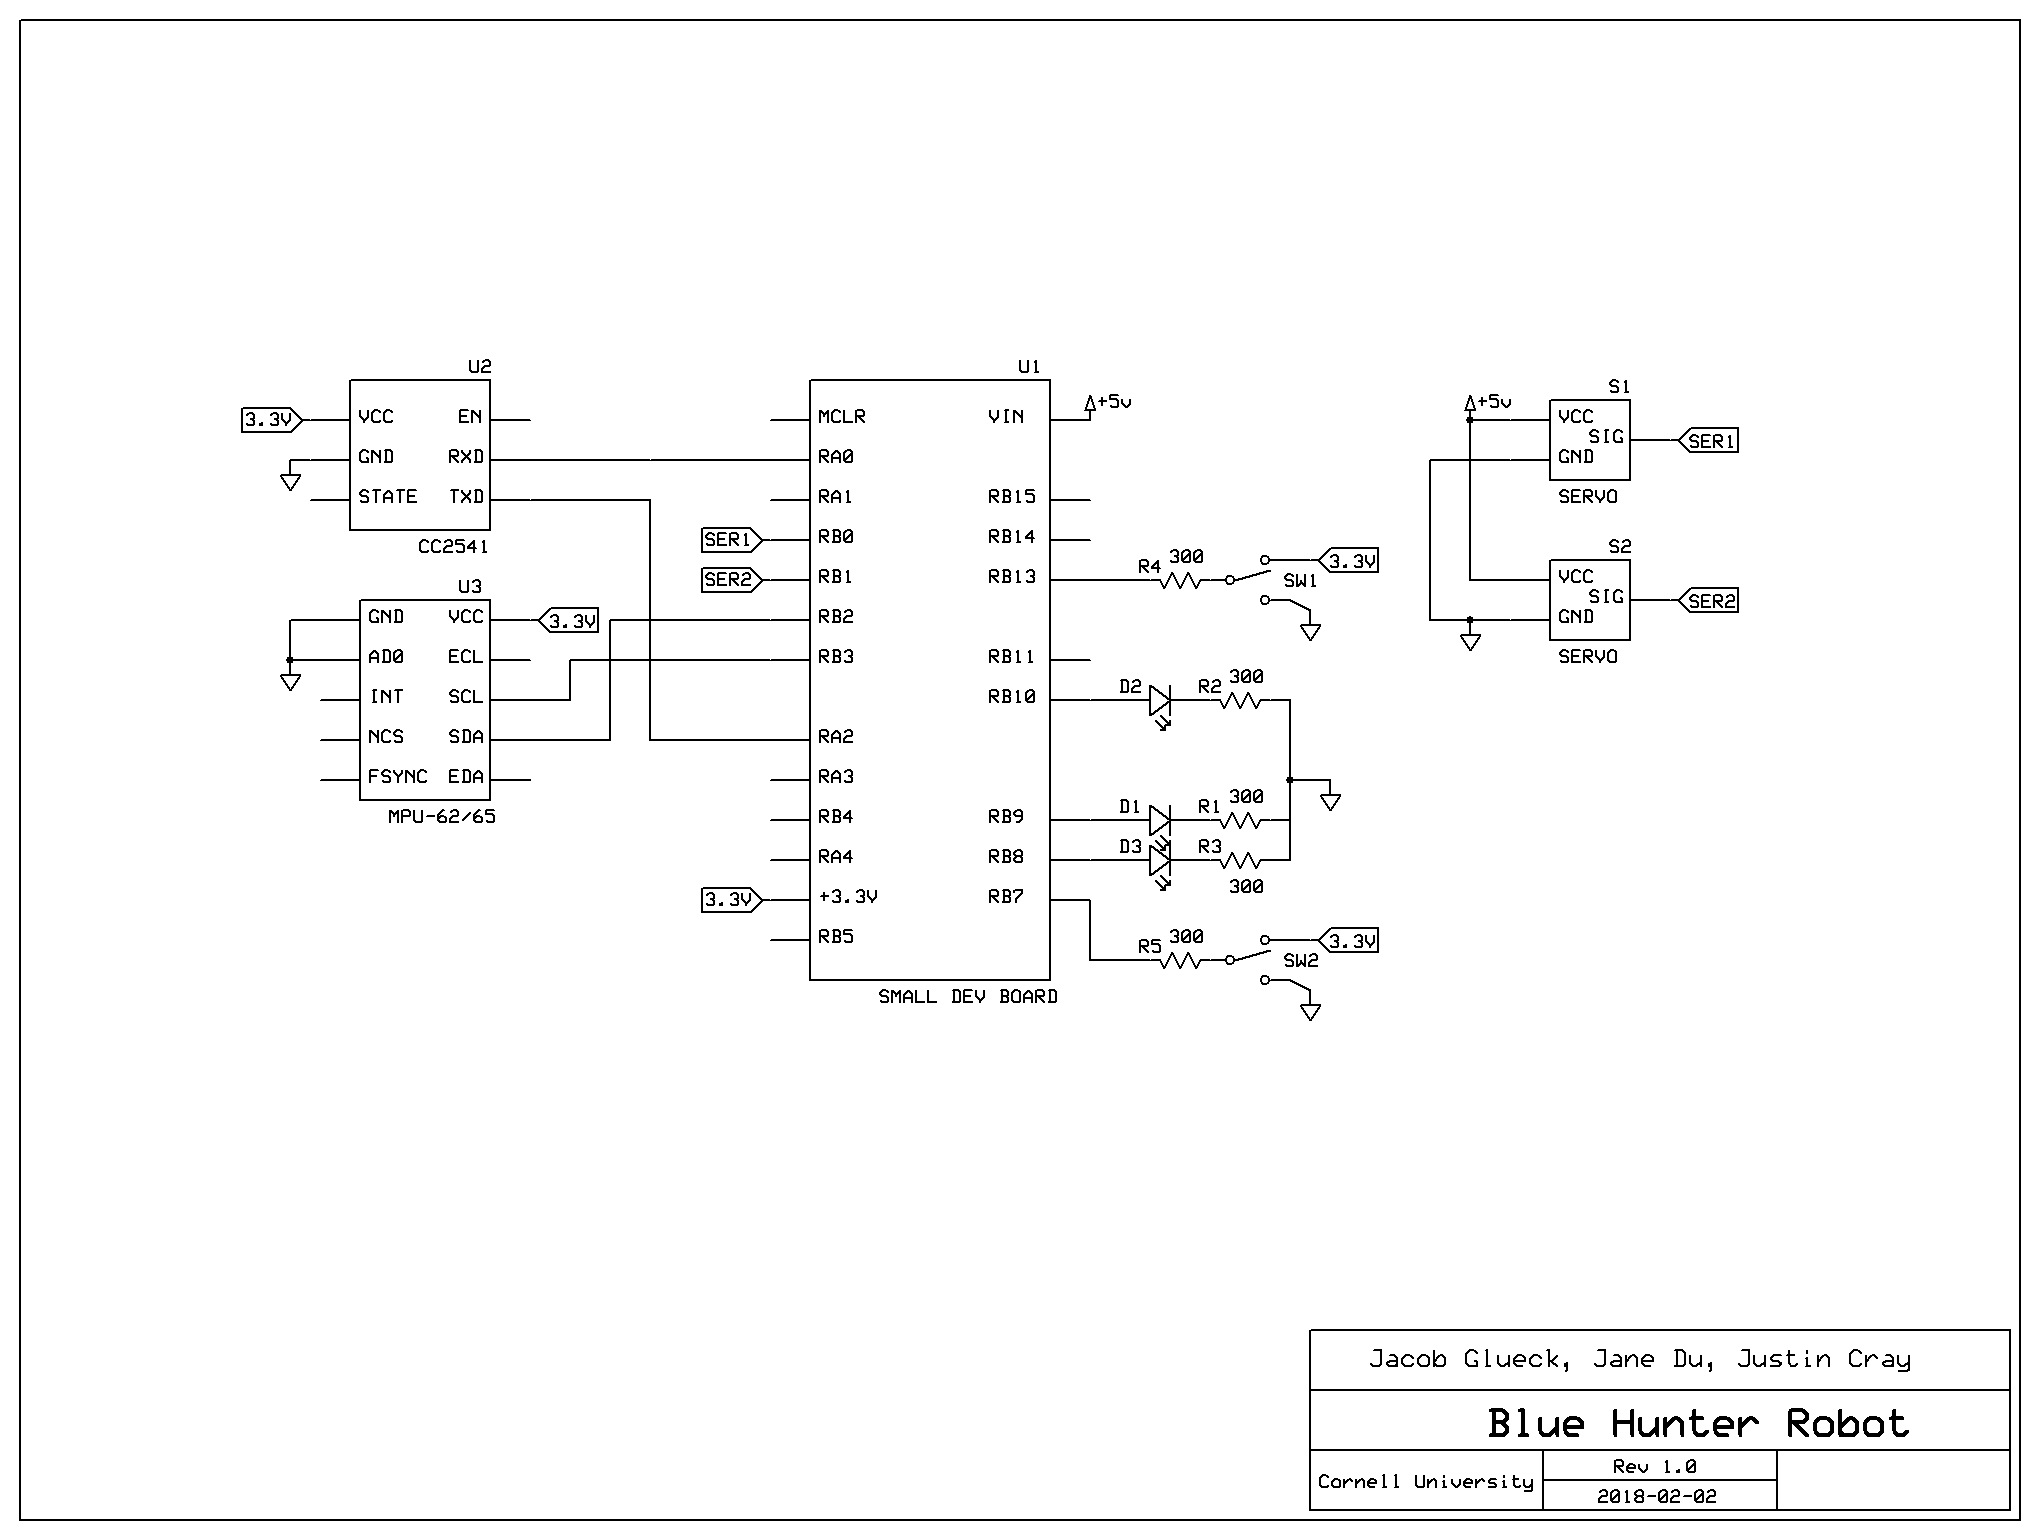
\includegraphics[width=0.9\textwidth]{bluehunters-robot.png}
  }
  \\
  \subfloat[] {
    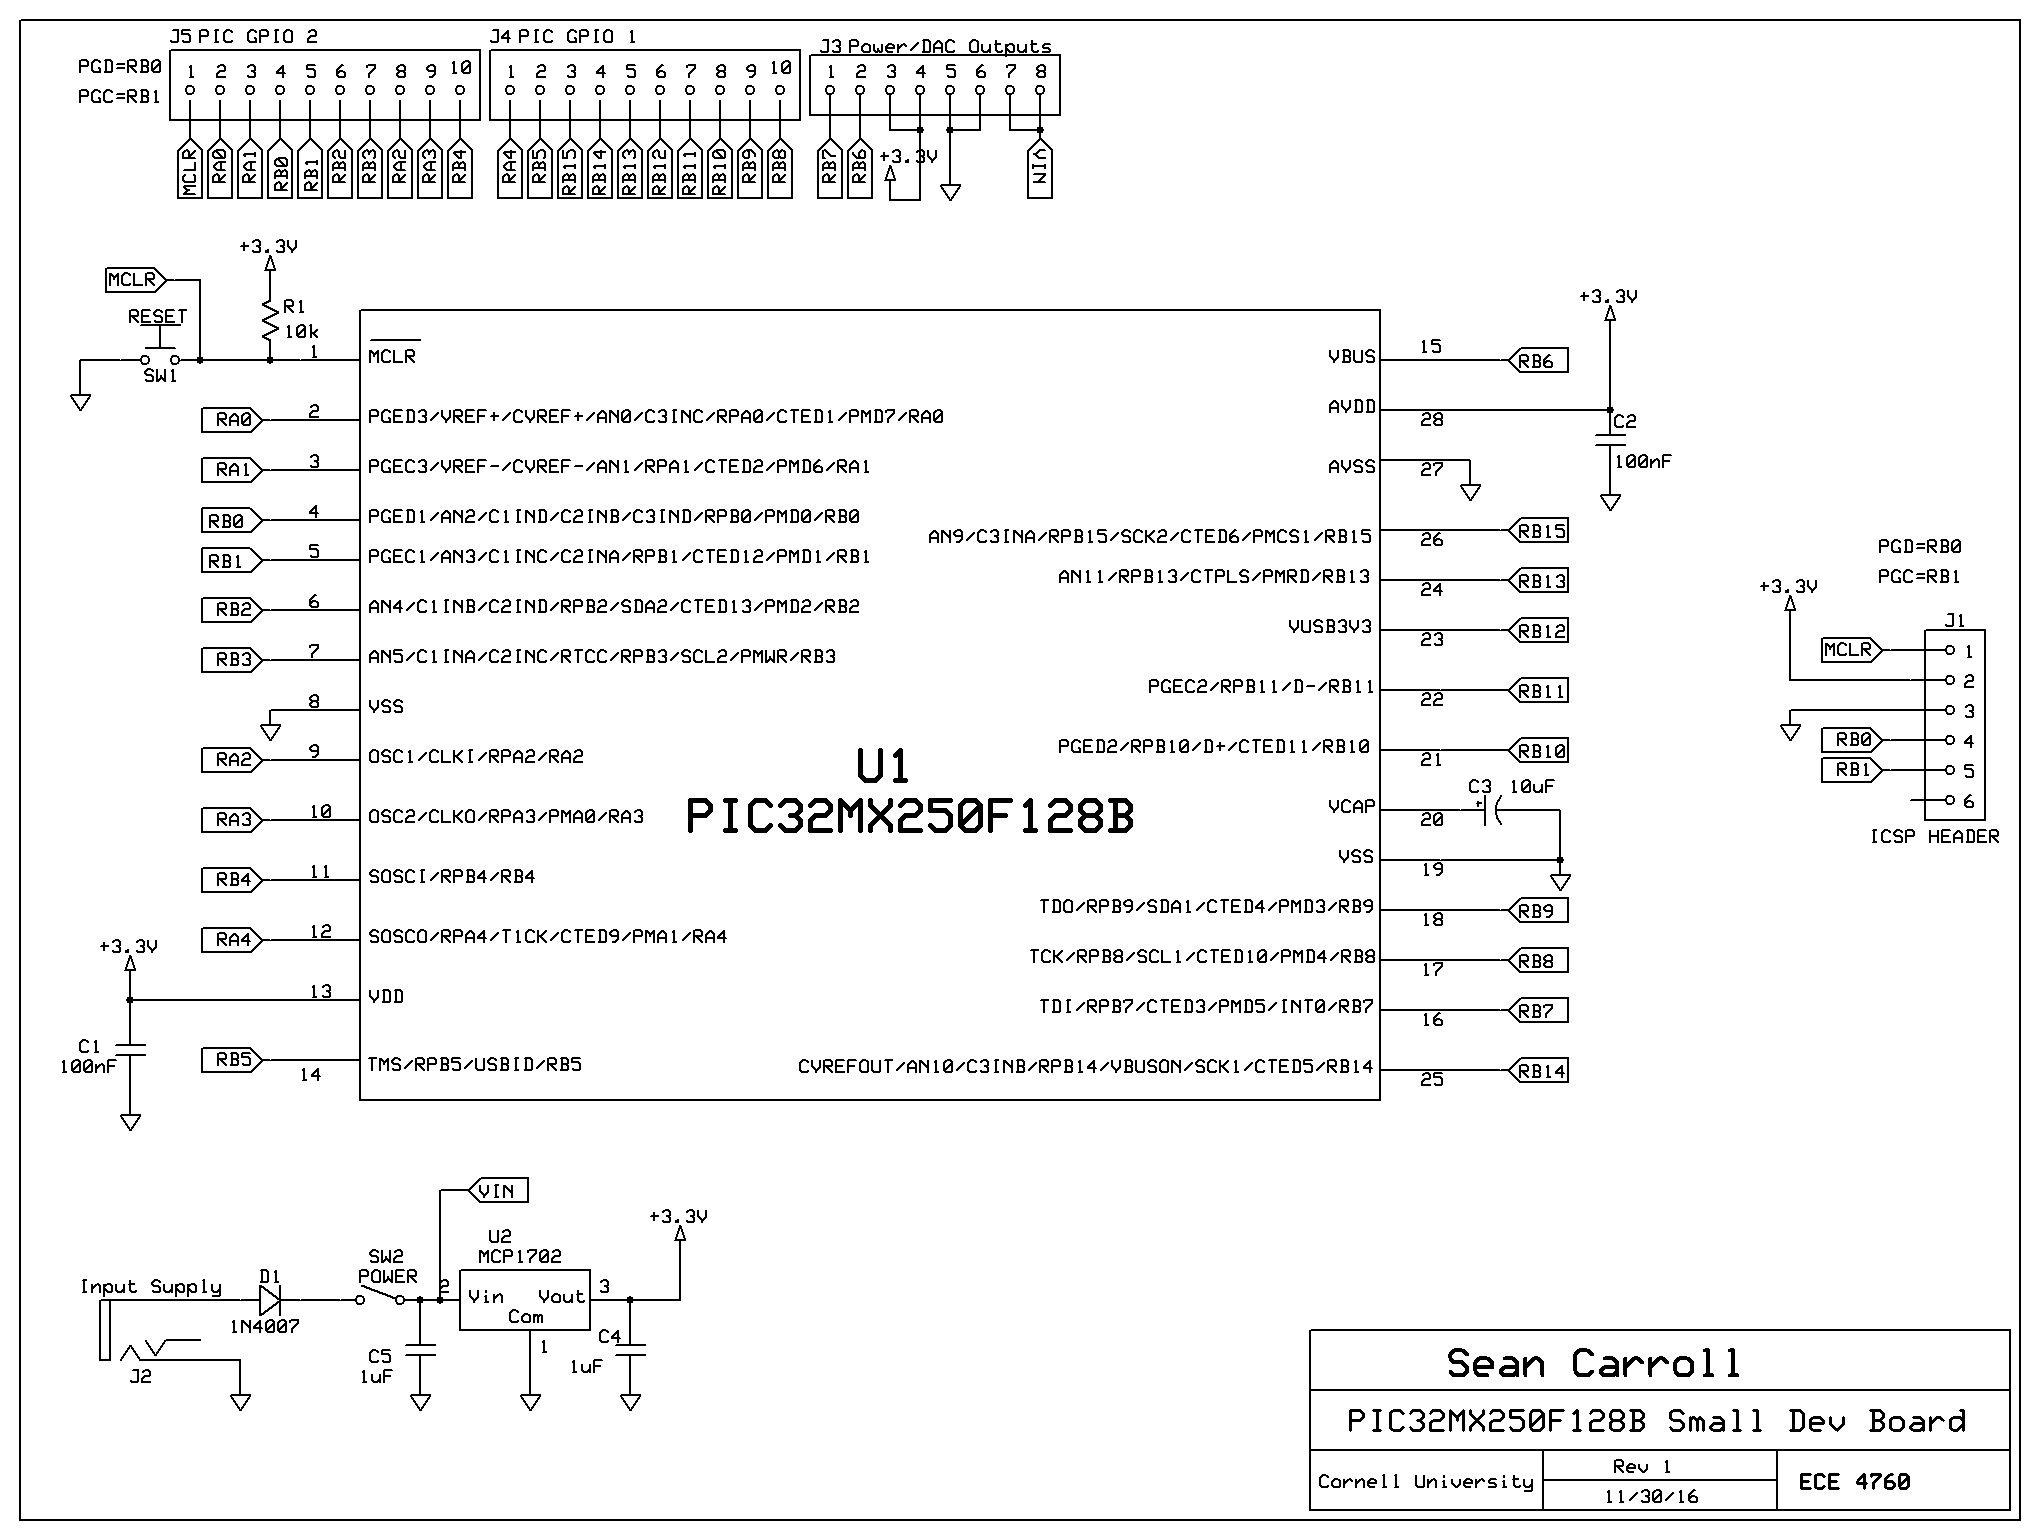
\includegraphics[width=0.9\textwidth]{bluehunters-sdb.png}
  }
  \caption{Schematic}
  \label{fig:schematic}
\end{figure}

\paragraph{Bluetooth modules}

The HM-10 bluetooth modules we bought off Ebay were fakes: they were not made by Jnhuamao,
\footnote{Jnhuamao is the company which makes the HM-10 module, along with other Bluetooth modules. Their English website is: \url{http://www.jnhuamao.cn/bluetooth.asp?id=1}.}
and did not come with genuine Jnhuamao firmware.
However, they did have genuine TI CC2541 chips.
We realized they were fakes when they did not behave according to
the Jnhuamao data sheet.
\footnote{The original data sheet comes from \cite{jnhuamaodatasheet}.
A PDF is available at \cite{jnhuamaomit}, which may be out of date, but is eaiser to get.}
Luckily, the hardware on the fake chips is the same as that of the genuine chips, minus an external crystal, and the genuine firmware checks for the presence of the crystal, and works even without
it. \cite{crystal}
As such, we reprogrammed the chips with the genuine firmware according
to an Arduino \cite{crystal}:

\begin{enumerate}
\item
  We soldered wires to the programming pins on the breakout boards, and connected those pins to an Arduino Teensy 3.2.
  We chose a Teensy because it is 3.3 volts as opposed to 5, which would damage the 3.3 volt CC2541. The pins were connected as follows:

  \begin{longtable}[]{@{}lll@{}}
  \toprule
  Name & CC2541 Pin & Arduino Pin\tabularnewline
  \midrule
  \endhead
  \texttt{DEBUG\_CLOCK} & 7 & 5\tabularnewline
  \texttt{DEBUG\_DATA} & 8 & 6\tabularnewline
  \texttt{RESET\_N} & 11 & 4\tabularnewline
  \bottomrule
  \end{longtable}

  Figure \ref{fig:hm10} shows the layout of the HM-10 module.
  \begin{figure}
    \centering
    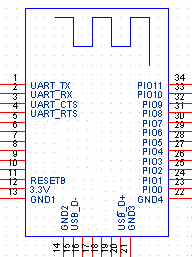
\includegraphics[width=0.3\textwidth]{hm10_pins.png}
    \caption{HM-10 module pin layout \cite{crystal}}
    \label{fig:hm10}
  \end{figure}

\item
  We uploaded the \texttt{CCLoader.ino} \cite{ccloader} sketch to the Arduino.
\item
  Finally, we ran (in a Windows virtual machine, due to the dubious origin of the software) \texttt{CCLoader.exe} \cite{ccloaderexe}.
  This program takes 3 arguments:

  \begin{Verbatim}[gobble=4]
    CCLoader.exe <COM Port> <Firmware.bin> 0
  \end{Verbatim}

  The firmware file came from the Arduino forum post \cite{crystal}, and can be
  found at \url{http://forum.arduino.cc/index.php?action=dlattach;topic=393655.0;attach=183702}.
\end{enumerate}

After flashing genuine firmware onto the chip, the next step was to update the firmware to the latest version.
The firmware flashed onto the board was version 540, but Jnhuamao had (at the time we did this project) released version 603. \cite{jnhuamao603}
Based on their instructions \cite{jnhuamaoinstructions}, we flashed our chips:

\begin{enumerate}
\item
  Connect the HM-10 module to a computer using a 3.3 V FTDI to USB
  adapter. Then, use PUTTY to establish a serial session (9600 baud,
  8N1). Send the chip \texttt{AT}; if it is connected properly, it will
  respond with \texttt{OK}.
\item
  Send the chip \texttt{AT+SBLUP} to put it in firmware update mode. It
  will respond with \texttt{OK+SBLUP}. Terminate the PUTTY session.
\item
  Run the \texttt{HMSoft.exe} program distributed in the firmware update
  download. We ran it in a Windows virtual machine because we did not
  trust it.
\item
  Select the proper port and firmware file using the software, and hit
  ``Load Image''. The software should handle the rest!
\item
  To make sure it worked, establish a serial connection again using
  PUTTY. Send \texttt{AT+VERS?} to query the chip for version
  information.
\end{enumerate}

\subsubsection{Software}

The robots were programmed in C, using MPLAB X IDE v4.0, the XC32 v1.4
compiler and the PIC 32 Legacy Peripheral Library (plib).
The full source code is available in online: \url{https://github.com/orangeturtle739/bluehunters/tree/master/ble.X}.

\paragraph{BLE}

The BLE module used UART, at 9600 baud 8N1. We used \texttt{UART1} on
the PIC for communicating with the BLE module, and used \texttt{UART2}
for communicating with the computer (for debugging).
We used the following commands to interact with the bluetooth chip:

\begin{itemize}
\item
  \texttt{AT+RESET}: resets the chip to ensure it is in a clean state
  before receiving other commands.
\item
  \texttt{AT+IBEA1}: enables the iBeacon functionality of the chip (sets
  it to 1; \texttt{AT+IBEA0} would disable it by setting it to 0). This
  allows the chip to be found with an RSSI scan. After setting the
  value, we query it with \texttt{AT+IBEA?} and send the result over the
  other serial port to a computer for debugging.
\item
  \texttt{AT+ROLE0} or \texttt{AT+ROLE1}: sets the role to either
  peripheral (0) or central (1). The base station is set to peripheral,
  and the 2 robots are set to central. Peripheral means the device will
  respond in inquiries from a central device. This allows it to be
  discovered during an RSSI scan. After setting the value, we query it
  with \texttt{AT+ROLE?} and send the result over the other serial port
  to a computer for debugging.
\item
  \texttt{AT+IMME0} or \texttt{AT+IMME1}: sets the work state of the
  device to either actively listening for Bluetooth signals (0), or only
  acting when it receives a serial command (1). Once again, the base
  station is set to 0: it needs to listen for signals and respond. The
  robots are set to 1, as the chips need to initiate scan requests when
  they receive the command over serial. After setting the value, we
  query it with \texttt{AT+IMME?} and send the result over the other
  serial port to a computer for debugging.
\item
  \texttt{AT+NAME\%s}: sets the name of the chip (which is visible when
  scanning) to \texttt{\%s} (For example, \texttt{AT+NAMEPIRATE} names
  the chip \texttt{PIRATE}). We give all the chips unique names to make
  debugging easier. After setting the value, we query it with
  \texttt{AT+NAME?} and send the result over the other serial port to a
  computer for debugging.
\item
  \texttt{AT+SHOW3}: configures the device to advertise both its name
  and RSSI when scanning.
\item
  \texttt{AT+ADDR?}: queries the device for its hardware address. We
  recorded the hardware device of each chip, as when doing RSSI scans,
  the results are reported by hardware address.
\item
  \texttt{AT+DISI?}: performed only on the robots, causing a discovery
  scan. The result of the scan is a bunch of lines of the form:

\begin{verbatim}
OK+DISC:00000000:00000000000000000000000000000000:
  0000000000:6832A3801EBE:-080
\end{verbatim}

  The second to last token, \texttt{6832A3801EBE}, is the hardware
  address of the discovered device, and the last token, \texttt{-080},
  is the measured RSSI. The chip will transmit a line for each device it
  finds (``line'' is a misnomer as it does not separate them with any
  characters), followed by \texttt{OK+DISCE}.
\end{itemize}

One interesting thing to note about the chip is that commands do not
have to end with newlines or carriage returns. However, if sent, the
chip will ignore them.

\paragraph{IMU}

The PIC communicates with the IMU via I2C.
The IMU includes a breakout board for the QFN MPU-9250 \cite{mpu9250datasheet} \cite{mpu9250regmap} module, which itself includes 2 dies.
One contains the 3-axis gyroscope and 3-axis accelerometer, which were not
used in this project, and the other die is the AK8963 3-axis
magnetometer (compass). \cite{ak8963cdatasheet}

It is connected to the rest of the MPU module via an auxiliary I2C bus,
so it is not connected to the MPU's main I2C bus by default. While the
accelerometer and gyroscope registers can be read after powering up the
IMU, the compass also needs pass-through mode to be enabled on the IMU
to make it an accessible slave on the I2C bus. We based our IMU code off of the \texttt{i2c\_helper.h} from the Self-Balancing Robot project. \cite{selfbalancingrobot} The AK8963 has several modes
of operation, and the chip must be set to power-down mode before
switching to other modes. We read compass values with single measurement
mode, as in figure \ref{fig:imu_single_measurement}.

\begin{figure}
  \centering
  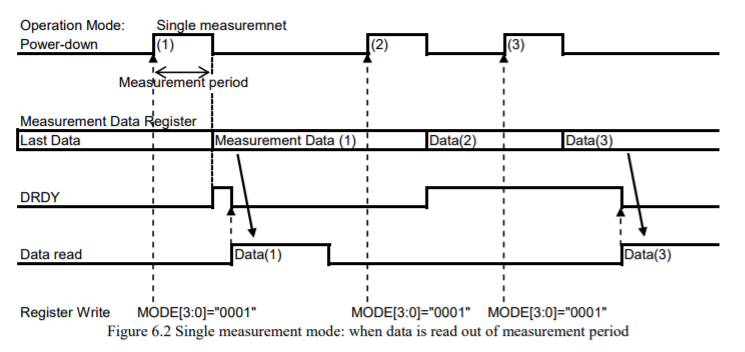
\includegraphics[width=0.9\textwidth]{imu_single_measurement.png}
  \caption{IMU single measurement mode}
  \label{fig:imu_single_measurement}
\end{figure}

In order to read the magnetometer, we:
\begin{enumerate}
\item
  Set the compass to single measurement mode in 14 bit resolution.
\item
  Read the 6 data registers (X low, X high, Y low, Y high, Z low, Z
  high)
\item
  Read the Status 2 register to check for magnetic sensor overflow.
  Without reading this register, the read is not considered complete and
  further reads will fail.
\item
  Wait; if the IMU is read too frequently, it will not have enough time
  to take measurements.
\end{enumerate}

In order to calibrate the compass, the robots spun in place when powered
on. They recorded the maximum and minimum values for each axes, and used
that data to scale and center the magnetometer readings.

\paragraph{Servos}

For the drive system, we used the FS90R servos. These servos are
continuous rotation servos with a stall torque of 1.5 kg-cm. Continuous
rotation servos operate based on PWM duty cycle; since servos operate at
a pulse width of 1 to 2 ms out of 20 ms, we used a timer with a
prescaler of 32 and a maximum count of 25600, and set the pwm at numbers
ranging from 1280 to 2560 (corresponding to the right pulse width).

A 50\% duty cycle means the servos are still. A less than 50\% duty
cycle means the servo turns clockwise and a greater than 50\% duty cycle
means the servo turns counter-clockwise. To implement the PWM, we use
the output capture on the PIC. We set the duty cycle using the built in
timers. We set a max and min duty cycle value which were experimentally
derived. The middle point is the average of the two. Tank drive is used
to control the system where both wheels are driven forward or point
turns where one wheel is turned in one direction and one is turned in
the other direction.

\paragraph{Gradient descent}

The algorithm for deciding what path to follow is a basic version of
gradient descent. Figure \ref{fig:graddesc} shows 2 versions of the gradient descent algorithm.

\begin{figure}
  \centering
  \subfloat[Simple gradient descent]{
    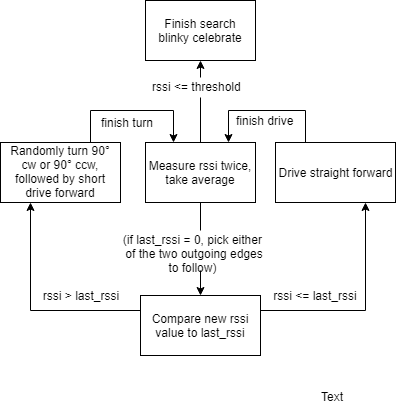
\includegraphics[width=0.4\textwidth]{grad_desc.png}
    \label{fig:simplegrad}
  }
  \subfloat[Compensating gradient descent]{
      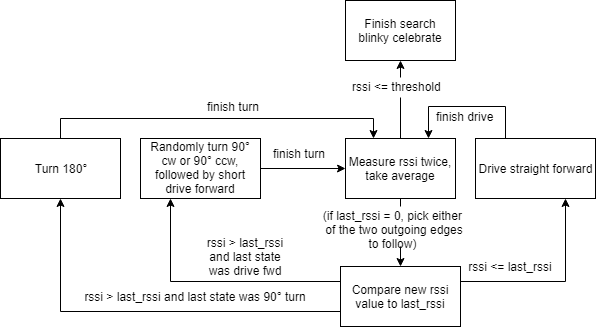
\includegraphics[width=0.5\textwidth]{turn_correction.png}
    \label{fig:simplegrad}
  }
  \caption{2 gradient descent algorithms. The initial state is \emph{measure RSSI twice, take average}.}
  \label{fig:graddesc}
\end{figure}

The purpose of the compensating algorithm was to allow the robots to recover faster after taking a wrong turn: if it just just moved forward and detected a
weakened signal, turned, and still detected a weaker signal, then it must have turned the wrong way, so it does a 180. However, it did not prove much more accurate than randomized gradient descent, largely due to noisy readings from IMU and Bluetooth signal strength. As such, we used the simplified version.

\subsection{Results}

In most cases, at least 1 of the 2 robots successfully made it to the
base station. However, it was not as reliable as we initially hoped. One
of the main reasons for this was the noise in RSSI measurements.

We expected that RSSI would vary with distance according to the
following relation:

\(\text{RSSI} = A - 10 n \log(d)\)

where \(A\) and \(n\) are RF propagation parameters in dBm, \(d\) is
distance in meters, and RSSI is the measured RSSI in dBm. \cite{5415423}
We experimented with RSSI measurements to determine how well they worked
by taking 2 Bluetooth modules, and measuring the RSSI while changing the
distance between them. One remained stationary on the floor and the
other was moved away from it 1 floor tile (each floor tile is a 1 foot
square) at a time. At each point, we took 3 RSSI measurements and
averaged them. Figure \ref{fig:rssiplot} shows the results (the original data is in table \ref{table:rssidata}).

\begin{figure}
  \centering
  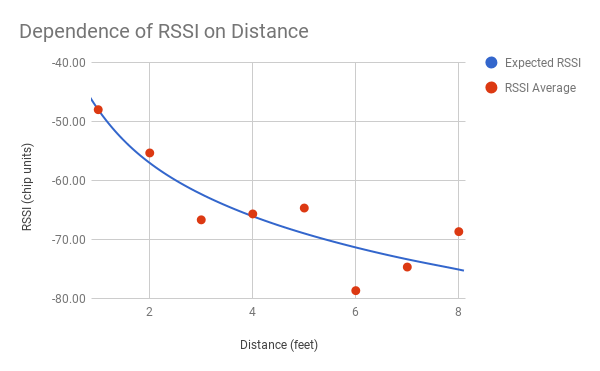
\includegraphics[width=0.9\textwidth]{rssi-chart.png}
  \caption{Plot showing bluetooth RSSI as a function of distance}
  \label{fig:rssiplot}
\end{figure}

\begin{table}
  \centering
  \begin{tabular}[]{@{}llllll@{}}
  \toprule
  Distance (feet) & RSSI A & RSSI B & RSSI C & RSSI Average & Expected
  RSSI \\
  \midrule
  1 & -48 & -48 & -48 & -48.00 & -48.00 \\
  2 & -56 & -58 & -52 & -55.33 & -57.03 \\
  3 & -66 & -66 & -68 & -66.67 & -62.31 \\
  4 & -64 & -68 & -65 & -65.67 & -66.06 \\
  5 & -60 & -70 & -64 & -64.67 & -68.97 \\
  6 & -80 & -80 & -76 & -78.67 & -71.34 \\
  7 & -80 & -79 & -65 & -74.67 & -73.35 \\
  8 & -68 & -66 & -72 & -68.67 & -75.09 \\
  \bottomrule
  \end{tabular}
  \caption{RSSI and distance data}
  \label{table:rssidata}
\end{table}

While the chip reported RSSI in units proportional to dBm, and we
measured distances in feet, not meters, we could still use the above
formula without worrying about unit conversions. The constants \(A\) and
\(n\), provided we determined them empirically based on the data, would
encode the conversions. As such, we fit the data using the above formula
with \(A=-48\) and \(n=3\), resulting in the blue curve above. While the
general shape of the curve matches, there is significant noise in the
averaged RSSI data. Furthermore, when we tried to reproduce the
measurements, we could not do so precisely -- it seemed to even depend
on where our feet where!

Despite how noisy the RSSI measurements where, the robots were still
able to perform a reasonably accurate gradient descent. In most cases,
at least one of the 2 robots would find the beacon in a matter of
minutes.

\subsection{Conclusions}

This project was an interesting exploration into short-range distance
determination using Bluetooth, a generally unconventional approach.
We knew that Bluetooth RSSI would be noisy, mostly due to multipath interference.
The robots worked reliably when they stayed within roughly 1 meter of the beacon.
After this, they entered the land of shallow gradients:
the signal strength from the beacon (already noisy) would not change very
much, and often only due to noise.
They normally could never recover from this.

There are many potential avenues for improvements or further
development:

\begin{itemize}
\tightlist
\item
  \emph{Communication between the two robots}. While Bluetooth may not
  offer good distance measurement via RSSI, it can be used for reliable
  communication between modules. It would be straightforward for one
  hunting robot to inform the other whether it believes it is
  approaching the beacon or not. In the simplest case, a hunting robot
  that is approaching, or already at, the beacon can provide a second
  point of reference for a currently hunting robot.
\item
  \emph{More complete usage of IMU}. Additional usage of the accelerometer and gyroscope, coupled with feedback from the servos, would allow the robots to maintain a dead-reckoning position estimate. This, paired with inter-swarm
  communication, would make for a much more sophisticated and likely
  much more efficient system. (Of course, this does not resolve the
  shallow gradients problem -- but it would allow the approach to the
  beacon to be much faster.)
\end{itemize}

\subsubsection{Appendix A: Bill Of Materials}

This project was done with a \$150 budget in mind. Costs for parts labeled ``Lab rental'' were borrowed from the department of Electrical and Computer Engineering at Cornell University, but can also be found at vendors like Digikey, Adafruit, and Amazon.

\begin{longtable}[]{@{}lllllll@{}}
\toprule
\begin{minipage}[b]{0.15\columnwidth}\raggedright
Name\strut
\end{minipage} & \begin{minipage}[b]{0.15\columnwidth}\raggedright
Manufacturer Part Number\strut
\end{minipage} & \begin{minipage}[b]{0.10\columnwidth}\raggedright
Vendor\strut
\end{minipage} & \begin{minipage}[b]{0.17\columnwidth}\raggedright
Vendor Part Number\strut
\end{minipage} & \begin{minipage}[b]{0.11\columnwidth}\raggedright
Quantity\strut
\end{minipage} & \begin{minipage}[b]{0.06\columnwidth}\raggedright
Unit Cost\strut
\end{minipage} & \begin{minipage}[b]{0.07\columnwidth}\raggedright
Total Cost\strut
\end{minipage}\tabularnewline
\midrule
\endhead
\begin{minipage}[t]{0.15\columnwidth}\raggedright
BLE 4.0 Module (TI CC2541)\strut
\end{minipage} & \begin{minipage}[t]{0.15\columnwidth}\raggedright
HM-10\strut
\end{minipage} & \begin{minipage}[t]{0.10\columnwidth}\raggedright
\href{https://www.ebay.com/itm/AT-09-BLE-Bluetooth-4-0-Uart-Transceiver-Module-CC2541-Central-Switching-HM-10/142425748901?ssPageName=STRK\%3AMEBIDX\%3AIT\&_trksid=p2057872.m2749.l2649}{Ebay}\strut
\end{minipage} & \begin{minipage}[t]{0.17\columnwidth}\raggedright
142425748901\strut
\end{minipage} & \begin{minipage}[t]{0.11\columnwidth}\raggedright
3\strut
\end{minipage} & \begin{minipage}[t]{0.06\columnwidth}\raggedright
\$3.99\strut
\end{minipage} & \begin{minipage}[t]{0.07\columnwidth}\raggedright
\$11.97\strut
\end{minipage}\tabularnewline
\begin{minipage}[t]{0.15\columnwidth}\raggedright
FEETECH FS90R (pack of 2) Continuous Rotation Robotic Servo\strut
\end{minipage} & \begin{minipage}[t]{0.15\columnwidth}\raggedright
FS90R\strut
\end{minipage} & \begin{minipage}[t]{0.10\columnwidth}\raggedright
\href{https://www.amazon.com/gp/product/B074BFQC3Q/ref=oh_aui_detailpage_o06_s00?ie=UTF8\&psc=1}{Amazon}\strut
\end{minipage} & \begin{minipage}[t]{0.17\columnwidth}\raggedright
B074BFQC3Q\strut
\end{minipage} & \begin{minipage}[t]{0.11\columnwidth}\raggedright
2\strut
\end{minipage} & \begin{minipage}[t]{0.06\columnwidth}\raggedright
\$12.39\strut
\end{minipage} & \begin{minipage}[t]{0.07\columnwidth}\raggedright
\$24.78\strut
\end{minipage}\tabularnewline
\begin{minipage}[t]{0.15\columnwidth}\raggedright
HiLetgo 9-Axis 9 DOF 16 Bit Gyroscope Acceleration Magnetic Sensor\strut
\end{minipage} & \begin{minipage}[t]{0.15\columnwidth}\raggedright
MPU-9250\strut
\end{minipage} & \begin{minipage}[t]{0.10\columnwidth}\raggedright
\href{https://www.amazon.com/HiLetgo-Gyroscope-Acceleration-Accelerator-Magnetometer/dp/B01I1J0Z7Y/ref=redir_mobile_desktop?_encoding=UTF8\&dpID=51nl2fcMh6L\&dpPl=1\&keywords=mpu\%209250\&pi=AC_SX236_SY340_QL65\&qid=1512564044\&ref=plSrch\&ref_=mp_s_a_1_3\&sr=8-3}{Amazon}\strut
\end{minipage} & \begin{minipage}[t]{0.17\columnwidth}\raggedright
B01I1J0Z7Y\strut
\end{minipage} & \begin{minipage}[t]{0.11\columnwidth}\raggedright
2\strut
\end{minipage} & \begin{minipage}[t]{0.06\columnwidth}\raggedright
\$8.49\strut
\end{minipage} & \begin{minipage}[t]{0.07\columnwidth}\raggedright
\$16.98\strut
\end{minipage}\tabularnewline
\begin{minipage}[t]{0.15\columnwidth}\raggedright
Small board\strut
\end{minipage} & \begin{minipage}[t]{0.15\columnwidth}\raggedright
--\strut
\end{minipage} & \begin{minipage}[t]{0.10\columnwidth}\raggedright
Lab rental\strut
\end{minipage} & \begin{minipage}[t]{0.17\columnwidth}\raggedright
--\strut
\end{minipage} & \begin{minipage}[t]{0.11\columnwidth}\raggedright
3\strut
\end{minipage} & \begin{minipage}[t]{0.06\columnwidth}\raggedright
\$5.00\strut
\end{minipage} & \begin{minipage}[t]{0.07\columnwidth}\raggedright
\$15.00\strut
\end{minipage}\tabularnewline
\begin{minipage}[t]{0.15\columnwidth}\raggedright
PIC32MX250F128B\strut
\end{minipage} & \begin{minipage}[t]{0.15\columnwidth}\raggedright
PIC32MX250F128B\strut
\end{minipage} & \begin{minipage}[t]{0.10\columnwidth}\raggedright
Lab rental\strut
\end{minipage} & \begin{minipage}[t]{0.17\columnwidth}\raggedright
--\strut
\end{minipage} & \begin{minipage}[t]{0.11\columnwidth}\raggedright
3\strut
\end{minipage} & \begin{minipage}[t]{0.06\columnwidth}\raggedright
\$5.00\strut
\end{minipage} & \begin{minipage}[t]{0.07\columnwidth}\raggedright
\$15.00\strut
\end{minipage}\tabularnewline
\begin{minipage}[t]{0.15\columnwidth}\raggedright
6-inch Protoboard\strut
\end{minipage} & \begin{minipage}[t]{0.15\columnwidth}\raggedright
--\strut
\end{minipage} & \begin{minipage}[t]{0.10\columnwidth}\raggedright
Lab rental\strut
\end{minipage} & \begin{minipage}[t]{0.17\columnwidth}\raggedright
--\strut
\end{minipage} & \begin{minipage}[t]{0.11\columnwidth}\raggedright
3\strut
\end{minipage} & \begin{minipage}[t]{0.06\columnwidth}\raggedright
\$2.50\strut
\end{minipage} & \begin{minipage}[t]{0.07\columnwidth}\raggedright
\$7.50\strut
\end{minipage}\tabularnewline
\begin{minipage}[t]{0.15\columnwidth}\raggedright
Male header pins\strut
\end{minipage} & \begin{minipage}[t]{0.15\columnwidth}\raggedright
--\strut
\end{minipage} & \begin{minipage}[t]{0.10\columnwidth}\raggedright
Lab\strut
\end{minipage} & \begin{minipage}[t]{0.17\columnwidth}\raggedright
--\strut
\end{minipage} & \begin{minipage}[t]{0.11\columnwidth}\raggedright
129\strut
\end{minipage} & \begin{minipage}[t]{0.06\columnwidth}\raggedright
\$0.05\strut
\end{minipage} & \begin{minipage}[t]{0.07\columnwidth}\raggedright
\$6.45\strut
\end{minipage}\tabularnewline
\bottomrule
\end{longtable}

\textbf{Total:} \$97.68

\bibliography{references}{}
\bibliographystyle{ieeetr}


\end{document}
